\section{Knowledge modelling for Information Retrieval}

\begin{frame}{Online OWL reasoning-based approach}

    An approach focusing on OWL.
    
    \begin{itemize}
        \item An Information Retrieval ontology.
        \item Push knowledge closer to the data.
        \item Model domain knowledge as linked sets of taxonomies. 
    \end{itemize}

\end{frame}

\begin{frame}{Knowledge modelling}

    \begin{figure} [H]
        \begin{center}
            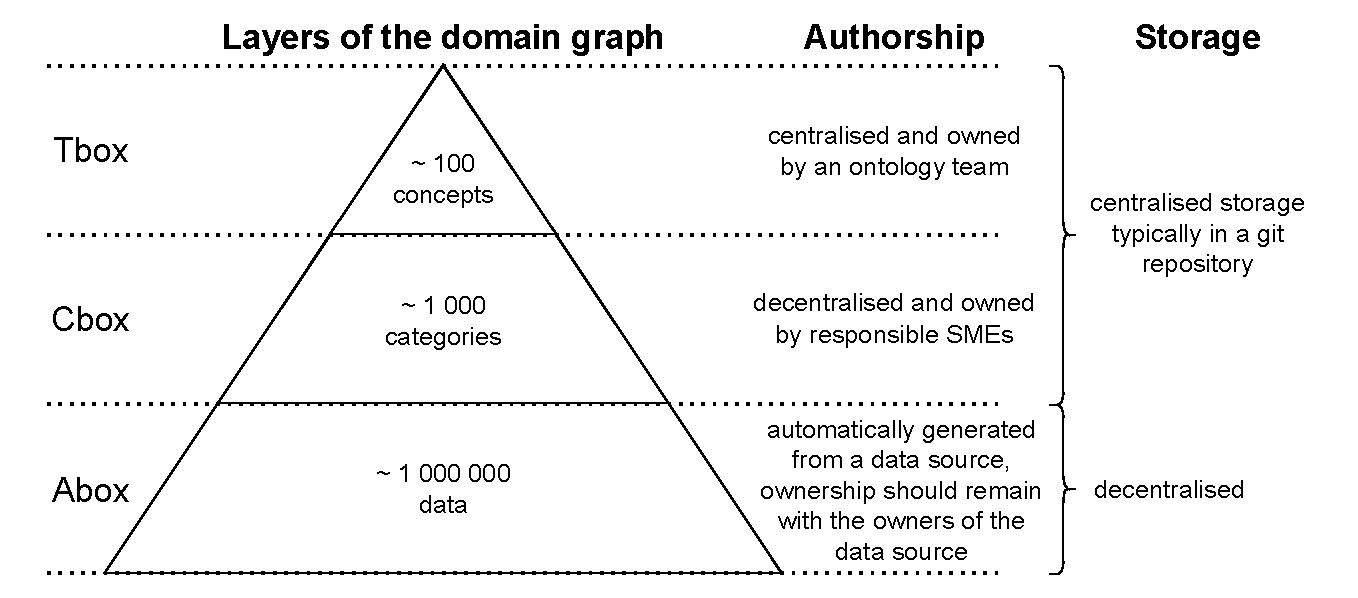
\includegraphics[scale=0.5]{images/TboxAboxCboxLayers.pdf} 
            \caption{"C-box" knowledge modelling approach} 
        \end{center}
    \end{figure}

\end{frame}

\begin{frame}{Information Retrieval Ontology}

    Competency questions:
    \begin{itemize}
        \item CQ1 What are the categories in the user search?
        \item CQ2 What are the documents relevant to a search?
        \item CQ3 What categories are enabled to refine the search?
    \end{itemize}

    7 classes:
    \begin{itemize}
        \item \emph{Candidate Document} subclass of \emph{Document} 
        \item \emph{Selected Category} and \emph{Enabled Category} subclasses of \emph{Category}
        \item \emph{Search Context} subclass of \emph{Search}
    \end{itemize}

    6 Object properties:
    \begin{itemize}
        \item \emph{categorises} inverse of \emph{categorised By}
        \item \emph{has Search Category} subproperty of \emph{enables Category}
        \item \emph{has Direct Subcategory} subproperty of \emph{has Subcategory}
    \end{itemize}

\end{frame}

\begin{frame}{Pizza ontology}

    Pizza ontology:
    \begin{itemize}
        \item Well-knowledge ontology built to introduce RDF/RDFS/OWL with examples (and even SHACL)
        \item Simple ontology with class hierarchies of:
        \begin{itemize}
            \item Pizzas (has topping, has base)
            \item Pizza bases
            \item Pizza Toppings
        \end{itemize} 
    \end{itemize}

    \begin{itemize}
        \item We use the Pizza ontology for demonstration in interest of time constraints 
    \end{itemize}

\end{frame}

\begin{frame}{Pizza ontology Knowledge Graph}

    \begin{figure} [H]
        \begin{center}
            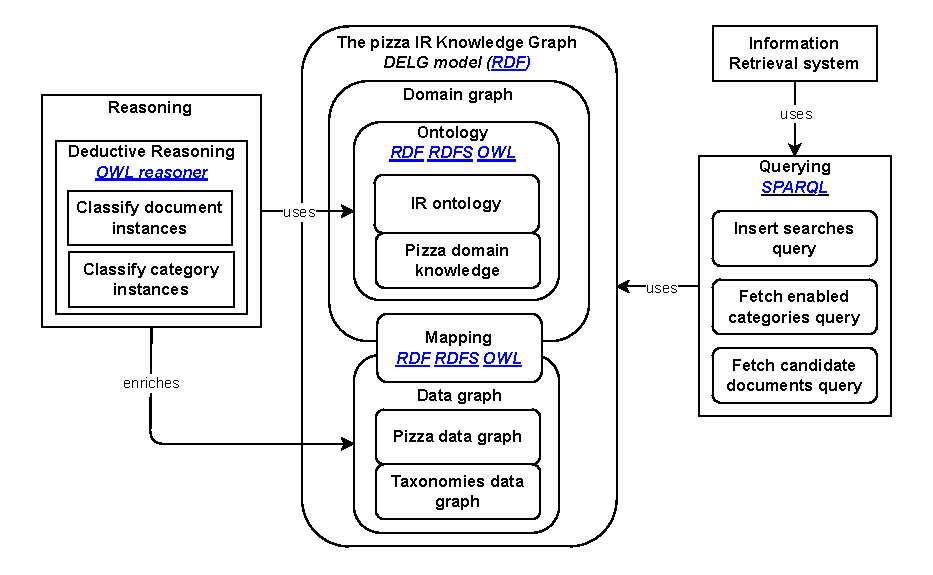
\includegraphics[scale=0.6]{images/pizza-demo-kg.pdf} 
            \caption{Pizza ontology Knowledge Graph} 
        \end{center}
    \end{figure}
\end{frame}


\begin{frame}{OWL reasoning-based Information Retrieval}

    \begin{figure} [H]
        \begin{center}
            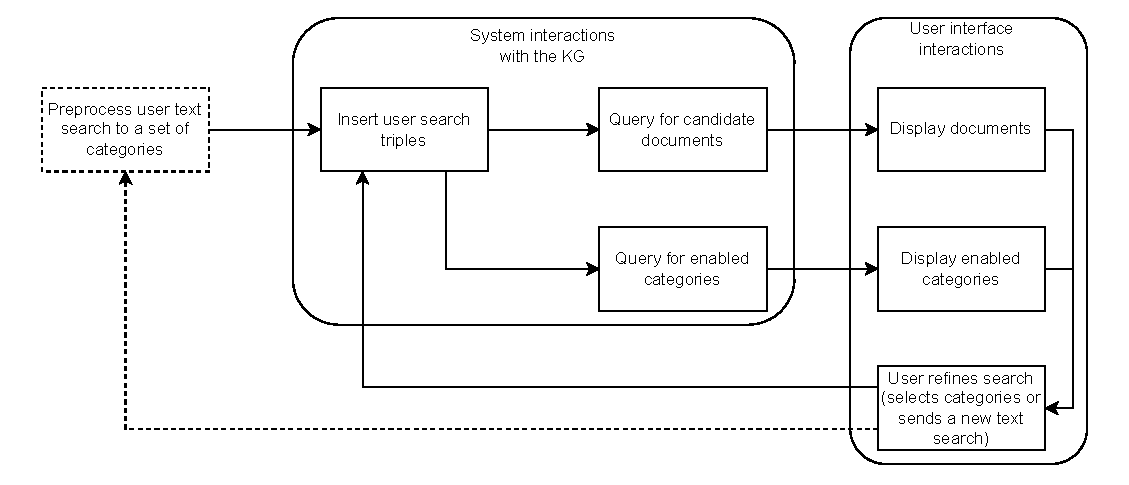
\includegraphics[scale=0.5]{images/ir-onto-search-process.pdf} 
            \caption{OWL reasoning-based Information Retrieval process.} 
        \end{center}
    \end{figure}
\end{frame}
